\documentclass[11pt]{article}

\usepackage[a4paper,margin=1in]{geometry}
\usepackage[T1]{fontenc}
\usepackage[utf8]{inputenc}
\usepackage{lmodern}
\usepackage{microtype}
\usepackage{amsmath,amssymb}
\usepackage{booktabs}
\usepackage{tabularx}
\usepackage{array}
\usepackage{longtable}
\usepackage{graphicx}
\usepackage{xcolor}
\usepackage{enumitem}
\usepackage{tikz}
\usetikzlibrary{arrows.meta,positioning,shapes.geometric,fit,calc}
\usepackage{url}
\usepackage[hidelinks]{hyperref}
\usepackage[nameinlink,noabbrev]{cleveref}
\usepackage{float}
\usepackage{listings}
\usepackage{fancyhdr}

\definecolor{traceblue}{RGB}{25,78,121}
\definecolor{tracegray}{RGB}{90,90,90}
\setlist{itemsep=2pt,topsep=3pt}
\setlength{\headheight}{14pt}
\pagestyle{fancy}
\fancyhf{}
\lhead{TRACE}
\rhead{Research paper}
\cfoot{\thepage}

\newcommand{\placeholder}[1]{\textcolor{red}{\textbf{[VERIFY: #1]}}}
\newcommand{\planned}[1]{\textcolor{tracegray}{\textit{[Planned evaluation: #1]}}}
\newcommand{\trace}[1]{\textsc{#1}}

\title{\textbf{TRACE: An AI-Assisted Geospatial Platform for Crime Reporting, Analysis, and Visualization}}
\author{Author name(s) to be supplied\\
\small Department and institution to be supplied\\
\small Corresponding author and e-mail to be supplied}
\date{\placeholder{Insert submission date}}

\begin{document}
\maketitle

\begin{abstract}
TRACE (Technology for Reporting, Analysis \& Crime Evaluation) is an
AI-assisted, map-oriented prototype for submitting, moderating, storing,
and exploring citizen incident reports. The system combines a React and
Leaflet client, a TypeScript/Express API, PostgreSQL with PostGIS, and a
Python FastAPI service. A report is validated, analysed from its narrative,
persisted with spatial coordinates, placed in a moderation workflow, and
made publicly visible only according to status and visibility rules. The
machine-learning component is a conventional text-classification prototype:
separate TF--IDF and Logistic Regression pipelines estimate incident category
and preliminary severity from synthetic, template-generated examples. It
does not use police records, observed crime outcomes, images, road-network
data, or a real-world labelled corpus. The map and analytics layers support
descriptive exploration of recorded reports; they should not be interpreted
as a causal or validated prediction of future crime or inherent neighbourhood
danger. This paper documents the verified implementation, its data model,
access-control and moderation design, and a reproducible evaluation plan.
Because no independent field study, labelled external test set, or measured
deployment benchmark was found in the supplied repository, numerical
effectiveness claims are intentionally not reported. The contribution is
therefore an inspectable prototype architecture and a clear specification of
the evidence required for future validation, including data-quality,
privacy, fairness, usability, security, and model-performance testing.
\end{abstract}

\noindent\textbf{Keywords:} crime reporting; geospatial information systems;
PostGIS; incident moderation; TF--IDF; Logistic Regression; decision support

\tableofcontents
\newpage

\section{Introduction}
\label{sec:introduction}

Citizens, moderators, and safety analysts often need to move from an
unstructured incident narrative to a record that can be searched by place,
reviewed by an authorised person, and presented in a form that supports
careful situational awareness. These tasks are difficult because a report
contains both textual and spatial information, reports may be incomplete or
duplicated, and a public map can create false certainty if reported events
are confused with the underlying incidence of crime. A useful system must
therefore combine data capture, validation, access control, spatial querying,
human review, and transparent presentation rather than treating a map marker
as a prediction.

TRACE is a prototype addressing this engineering problem. The repository
implements a map-first React interface, an Express and TypeScript backend,
PostgreSQL/PostGIS persistence, Socket.IO events, and a Python FastAPI
classification service. Its intended workflow is
\emph{report, validate, analyse, store, review, publish, and explore}.
Reports are initially non-public and are made visible according to
moderation state. The system also includes community corroboration and audit
records. These features make TRACE a decision-support and safety-awareness
prototype, not a replacement for emergency services, police records, or
official case adjudication.

This paper makes four boundaries explicit. First, crime reporting is not the
same as crime occurrence: the database represents submitted and moderated
reports. Second, map aggregation is descriptive visualization, not automatic
future-event prediction. Third, the AI service supplies preliminary signals
from text and does not establish that a reported event occurred. Fourth, the
available evidence does not verify operational deployment or independent
predictive performance.

\subsection{Objectives and research questions}
\label{sec:rqs}

The study is organized around the following questions:
\begin{enumerate}
  \item \textbf{RQ1:} How can a unified workflow connect citizen incident
  reporting, human moderation, spatial persistence, and public map
  visualization?
  \item \textbf{RQ2:} How can a conventional text-classification component
  provide transparent preliminary category and severity signals without
  being presented as ground truth?
  \item \textbf{RQ3:} What evaluation evidence is required to establish
  functional correctness, spatial-query performance, usability, security,
  fairness, and model validity for TRACE?
\end{enumerate}

\subsection{Contributions and scope}

The substantiated contributions are: (i) an implemented layered prototype;
(ii) a schema that combines relational, spatial, moderation, AI-analysis,
notification, audit, and corroboration entities; (iii) an explicit
moderation-to-visibility workflow; (iv) a reproducible description of the
synthetic text-classification mechanism; and (v) an evaluation protocol that
separates measured results from pending experiments. Claims of superiority,
police integration, automated dispatch, validated crime prediction, or
production deployment are outside the evidence available for this paper.

\section{Problem Statement and Motivation}
\label{sec:problem}

The engineering problem is to manage a report lifecycle in which a person
submits a narrative and location, the service derives structured assistance
signals, a moderator reviews the report, and the resulting state is exposed
to different audiences. The system must preserve a connection between the
original report and its AI analysis while preventing unreviewed data from
being silently presented as public fact.

The design has five related challenges:
\begin{enumerate}
  \item \textbf{Heterogeneous input:} narratives, categories, timestamps, and
  coordinates have different validation and storage needs.
  \item \textbf{Spatiotemporal exploration:} map queries need spatial indexes,
  filtering, clustering, and temporal fields.
  \item \textbf{Human oversight:} a moderator must be able to inspect and
  change lifecycle state, with an audit trail.
  \item \textbf{Uncertainty:} text classification is a preliminary signal
  whose confidence depends on a synthetic training distribution.
  \item \textbf{Responsible visibility:} rejected or under-review reports
  should not remain visible on the public map merely because they were once
  submitted.
\end{enumerate}

These challenges motivate a design in which database state, moderation rules,
and client-side real-time state are updated together. They also motivate
careful language: a concentration of reports may indicate reporting,
coverage, or enforcement patterns as well as underlying events.

\section{Background and Technical Foundations}
\label{sec:background}

\subsection{Digital incident reporting and GIS}

Digital reporting systems transform a narrative into a record that can be
searched, filtered, and audited. A geographic information system (GIS)
adds a spatial reference to that record. In TRACE, a report stores a
PostGIS point using WGS84/SRID 4326, together with denormalized latitude and
longitude fields. This supports map rendering and spatial predicates while
retaining ordinary relational attributes.

\subsection{Spatial visualization}

A point map displays individual records. Clustering groups nearby markers for
readability, while a heatmap or density layer aggregates points into visual
intensity. Such visualizations are descriptive transformations of the
selected data and settings. They do not, by themselves, estimate future
incidents, establish causality, or measure inherent danger. TRACE uses
Leaflet, marker clustering, and a heatmap dependency; the exact runtime
weighting and bandwidth configuration should be recorded from the deployed
client before a formal visualization study.

\subsection{Text classification}

TRACE's AI service uses a standard supervised text-classification pipeline.
TF--IDF maps cleaned unigrams and bigrams to numeric features. Logistic
Regression then computes class scores from learned coefficients and converts
them into class probabilities. The category and severity pipelines are
separate and have separate vectorizers. The model output is therefore
conventional machine learning, not random generation and not deep learning.

\subsection{Human-in-the-loop decision support}

Human review is important when labels concern public safety. In TRACE, the
classifier supplies a preliminary category, severity, and confidence;
moderators retain control over publication state. This does not remove bias:
the training labels, reporting population, language, and moderation practices
can all shape the resulting data.

\section{Related Work and Research Gap}
\label{sec:related}

Prior research on crime mapping shows the value of spatial representations
for exploratory analysis, while also warning that recorded incidents are
not a neutral sample of all events. Methodological work on kernel-density
estimation and spatial statistics provides useful tools for describing
concentration, but descriptive concentration should not be conflated with
causal explanation. Research on algorithmic crime prediction further
highlights feedback loops, unequal reporting, and the risks of automating
consequential decisions. Privacy research on location data motivates
minimization, access control, aggregation, and careful disclosure.

The defensible gap for TRACE is narrow: the project implements a small,
inspectable workflow that connects citizen narrative capture, AI-assisted
triage, PostGIS storage, moderator-controlled public visibility,
corroboration, and map exploration in one prototype. This is an integration
and evaluation subject, not a claim that no comparable system exists.

\begin{table}[H]
\centering
\caption{Analytical comparison of relevant approaches and TRACE's response.}
\label{tab:gap}
\small
\begin{tabularx}{\textwidth}{p{0.20\textwidth}p{0.22\textwidth}p{0.25\textwidth}X}
\toprule
\textbf{Approach} & \textbf{Strength} & \textbf{Limitation relevant here} & \textbf{TRACE response}\\
\midrule
Static point map & Simple spatial inspection & Can expose unreviewed or noisy records & Status and public-visibility fields gate map exposure\\
Density or heatmap visualization & Communicates concentration & Can be mistaken for prediction or danger & Paper labels it descriptive and requires controlled visualization tests\\
Text classifier & Reduces manual structuring effort & Depends on labels, language, and distribution & Separate TF--IDF/Logistic Regression signals are shown as preliminary\\
Fully automated classification & Fast triage & Weak contestability for sensitive decisions & Moderator review remains in the lifecycle\\
Relational incident store & Consistent records and constraints & Requires spatial extensions for GIS queries & PostgreSQL/PostGIS and GiST indexes support spatial access\\
Public reporting map & Improves situational awareness & Privacy and stigmatization risks & Authentication, role separation, anonymization goals, and ethical limits are documented\\
\bottomrule
\end{tabularx}
\end{table}

\section{Research Questions, Requirements, and Scope}
\label{sec:requirements}

\subsection{Actors and permissions}

The database defines three roles: \texttt{CITIZEN}, \texttt{MODERATOR}, and
\texttt{ADMIN}. Citizens submit incidents and corroborations and view
publicly eligible information. Moderators review reports and change status.
Administrators manage users, system statistics, and audit records. Exact
endpoint authorization is enforced in route middleware and should be
rechecked whenever a deployment configuration changes.

\begin{table}[H]
\centering
\caption{Requirements traceability from intended behavior to repository evidence.}
\label{tab:req}
\small
\begin{tabularx}{\textwidth}{p{0.12\textwidth}p{0.38\textwidth}p{0.30\textwidth}X}
\toprule
\textbf{ID} & \textbf{Requirement} & \textbf{Evidence} & \textbf{Status}\\
\midrule
R1 & Authenticated users can submit an incident narrative and location & Incident route, validation, incident controller, schema & Implemented; runtime regression should remain part of CI\\
R2 & Store a spatial point and query map data & PostGIS geometry, GiST index, map controller & Implemented\\
R3 & Analyse narrative category and severity & FastAPI service and saved joblib pipelines & Implemented prototype\\
R4 & Prevent unreviewed reports from public visibility & \texttt{status} and \texttt{is\_public} fields plus moderation controller & Implemented; deployment test required\\
R5 & Maintain human review and auditability & Moderator routes, audit logs, status transitions & Implemented\\
R6 & Support corroboration and credibility signals & Corroboration table, routes, controller, notifications & Implemented\\
R7 & Demonstrate real-world predictive validity & No labelled external dataset or experiment artifacts found & Not established\\
R8 & Demonstrate operational performance and usability & No benchmark or user-study artifacts found & Planned evaluation\\
\bottomrule
\end{tabularx}
\end{table}

\section{Proposed System: TRACE}
\label{sec:system}

\subsection{System overview}

The verified stack consists of React and Vite on the client; Leaflet,
marker-clustering, and a heatmap library for the map; Node.js, Express, and
TypeScript for the API; PostgreSQL and PostGIS for persistence; Socket.IO
for real-time events; and Python FastAPI with scikit-learn for text
analysis. The repository also includes a safe-route feature plan and
implementation surface, but this paper treats route-risk effectiveness as
unverified because no routing benchmark or independent road-risk dataset was
found.

\begin{figure}[H]
\centering
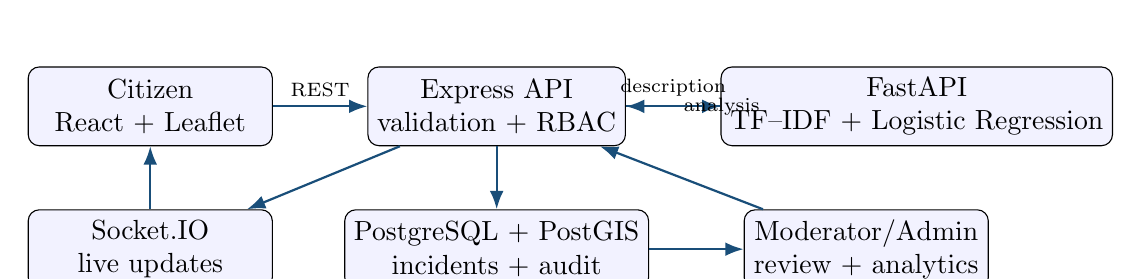
\begin{tikzpicture}[
  node distance=8mm and 12mm,
  box/.style={draw, rounded corners, align=center, minimum width=31mm, minimum height=10mm, fill=blue!5},
  arrow/.style={-Latex, thick, draw=traceblue}
]
\node[box] (citizen) {Citizen\\React + Leaflet};
\node[box,right=of citizen] (api) {Express API\\validation + RBAC};
\node[box,right=of api] (ai) {FastAPI\\TF--IDF + Logistic Regression};
\node[box,below=of api] (db) {PostgreSQL + PostGIS\\incidents + audit};
\node[box,right=of db] (mod) {Moderator/Admin\\review + analytics};
\node[box,below=of citizen] (socket) {Socket.IO\\live updates};
\draw[arrow] (citizen) -- node[above,font=\scriptsize]{REST} (api);
\draw[arrow] (api) -- node[above,font=\scriptsize]{description} (ai);
\draw[arrow] (ai) -- node[right,font=\scriptsize]{analysis} (api);
\draw[arrow] (api) -- (db);
\draw[arrow] (db) -- (mod);
\draw[arrow] (api) -- (socket);
\draw[arrow] (socket) -- (citizen);
\draw[arrow] (mod) -- (api);
\end{tikzpicture}
\caption{Verified high-level TRACE architecture. External police integration and operational deployment are not shown because they were not evidenced.}
\label{fig:architecture}
\end{figure}

\subsection{Report lifecycle}

The report lifecycle is:
\begin{enumerate}
  \item A citizen selects a map location and submits a narrative.
  \item The API validates the request and calls the AI service.
  \item The incident and analysis are persisted using database transactions.
  \item The initial record is non-public and enters moderation.
  \item A moderator changes the lifecycle state and visibility.
  \item Eligible records are returned by public map queries and can generate
  real-time client updates.
  \item Citizens may corroborate an eligible incident; the resulting score
  and notification are persisted.
\end{enumerate}

\begin{figure}[H]
\centering
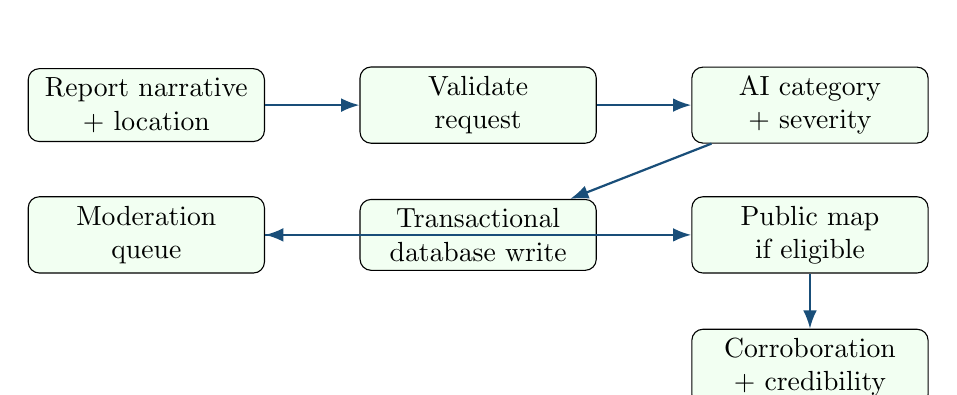
\begin{tikzpicture}[
  node distance=7mm and 12mm,
  box/.style={draw, rounded corners, align=center, minimum width=30mm, minimum height=9mm, fill=green!5},
  arrow/.style={-Latex, thick, draw=traceblue}
]
\node[box] (report) {Report narrative\\+ location};
\node[box,right=of report] (validate) {Validate\\request};
\node[box,right=of validate] (analyse) {AI category\\+ severity};
\node[box,below=of validate] (persist) {Transactional\\database write};
\node[box,left=of persist] (queue) {Moderation\\queue};
\node[box,right=of persist] (public) {Public map\\if eligible};
\node[box,below=of public] (corr) {Corroboration\\+ credibility};
\draw[arrow] (report) -- (validate);
\draw[arrow] (validate) -- (analyse);
\draw[arrow] (analyse) -- (persist);
\draw[arrow] (persist) -- (queue);
\draw[arrow] (queue) -- (public);
\draw[arrow] (public) -- (corr);
\end{tikzpicture}
\caption{Report lifecycle implemented by the application. Publication is a moderation outcome, not an automatic consequence of submission.}
\label{fig:lifecycle}
\end{figure}

\subsection{Map and analytics}

The map API exposes incident, cluster, heatmap, and nearby queries. The
database schema includes a GiST spatial index on the geometry column and
indexes on status, category, severity, user, and timestamps. These choices
support the intended exploratory workload. The application uses OpenStreetMap
tiles through Leaflet attribution; this is a map-tile dependency, not
evidence that an OSM road graph or validated road vulnerability model is
implemented.

\section{System Architecture and Design}
\label{sec:architecture}

\subsection{Layered design}

The presentation layer renders map markers, filters, report forms,
moderation queues, admin views, and corroboration interactions. The service
layer validates requests, applies authorization, calls the AI service, and
coordinates database transactions. The persistence layer stores normalized
entities and spatial geometry. The AI component is deliberately separated
as a Python service, allowing its model artifact and preprocessing to be
versioned independently.

\subsection{Report submission sequence}

\begin{figure}[H]
\centering
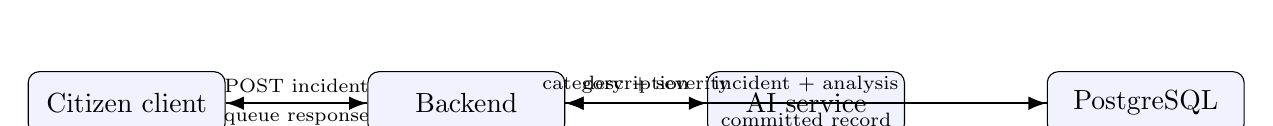
\begin{tikzpicture}[
  actor/.style={draw, rounded corners, fill=blue!5, minimum width=25mm, minimum height=8mm, align=center},
  msg/.style={-Latex, thick},
  node distance=13mm and 18mm
]
\node[actor] (u) {Citizen client};
\node[actor,right=of u] (b) {Backend};
\node[actor,right=of b] (a) {AI service};
\node[actor,right=of a] (d) {PostgreSQL};
\draw[msg] (u) -- node[above,font=\scriptsize]{POST incident} (b);
\draw[msg] (b) -- node[above,font=\scriptsize]{description} (a);
\draw[msg] (a) -- node[above,font=\scriptsize]{category + severity} (b);
\draw[msg] (b) -- node[above,font=\scriptsize]{incident + analysis} (d);
\draw[msg] (d) -- node[below,font=\scriptsize]{committed record} (b);
\draw[msg] (b) -- node[below,font=\scriptsize]{queue response} (u);
\end{tikzpicture}
\caption{Simplified report-submission sequence. Error handling and authorization are omitted from the drawing for readability but are part of the implementation.}
\label{fig:submission}
\end{figure}

\subsection{Map-analysis sequence}

\begin{figure}[H]
\centering
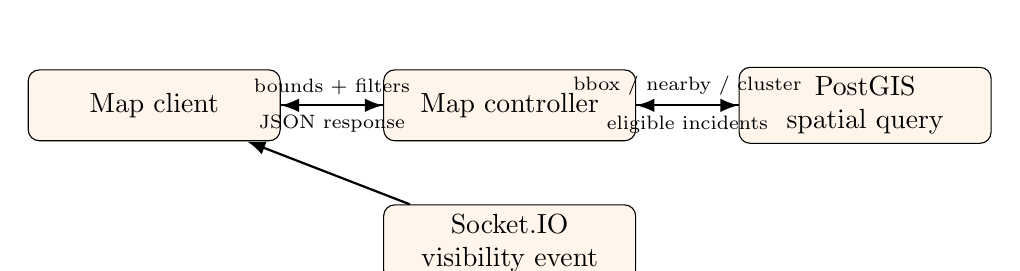
\begin{tikzpicture}[
  box/.style={draw, rounded corners, fill=orange!8, minimum width=32mm, minimum height=9mm, align=center},
  arr/.style={-Latex, thick},
  node distance=8mm and 13mm
]
\node[box] (client) {Map client};
\node[box,right=of client] (api) {Map controller};
\node[box,right=of api] (db) {PostGIS\\spatial query};
\node[box,below=of api] (socket) {Socket.IO\\visibility event};
\draw[arr] (client) -- node[above,font=\scriptsize]{bounds + filters} (api);
\draw[arr] (api) -- node[above,font=\scriptsize]{bbox / nearby / cluster} (db);
\draw[arr] (db) -- node[below,font=\scriptsize]{eligible incidents} (api);
\draw[arr] (api) -- node[below,font=\scriptsize]{JSON response} (client);
\draw[arr] (socket) -- (client);
\end{tikzpicture}
\caption{Map-query sequence with public eligibility applied by the API/database query layer.}
\label{fig:mapsequence}
\end{figure}

\section{Data Model and Data Management}
\label{sec:data}

\subsection{Entities}

The canonical schema defines users, incidents, incident media, incident
analysis, notifications, audit logs, and corroborations. Incidents reference
users and contain both a PostGIS point and denormalized coordinates. AI
analysis is linked one-to-many through an incident identifier. Moderation
notes are separate from public narrative content. Corroboration updates a
credibility score that is stored on the incident.

\begin{table}[H]
\centering
\caption{Selected schema entities and their roles.}
\label{tab:schema}
\small
\begin{tabularx}{\textwidth}{p{0.22\textwidth}p{0.28\textwidth}X}
\toprule
\textbf{Entity} & \textbf{Confirmed fields/concepts} & \textbf{Purpose}\\
\midrule
\texttt{users} & UUID, name, email, password hash, role, active flag, timestamps & Identity and role-based access\\
\texttt{incidents} & description, category, AI category/confidence, severity, status, geometry, coordinates, occurred time, public flag & Core report and lifecycle state\\
\texttt{incident\_analysis} & predicted category/severity, confidence, model version, processing time & Immutable-ish record of AI output\\
\texttt{incident\_media} & incident reference, URL, type, size, original name & Optional evidence metadata\\
\texttt{corroborations} & incident/user references and corroboration content/score fields & Community support signal\\
\texttt{notifications} & recipient, incident, type, title, message, read state & User-facing state changes\\
\texttt{audit\_logs} & actor, action, entity, metadata, IP/user-agent, timestamp & Accountability and investigation\\
\bottomrule
\end{tabularx}
\end{table}

\subsection{Data provenance and quality}

The report data is user-entered and seeded demo data; the repository does
not establish a representative population sample or an official crime
database. Coordinates are validated at the API boundary and stored as
WGS84 points. Potential quality issues include inaccurate pins, missing
details, duplicate reports, temporal ambiguity, underreporting, and
adversarial or malicious submissions. A production study would require
documented retention, deletion, consent, provenance, access review, backup,
and incident-response policies.

\section{AI, Classification, and Geospatial Analytics}
\label{sec:ai}

\subsection{Training data construction}

The supplied training script defines ten incident categories and manually
associates each category with a severity label. It expands template
sentences over a list of Pune-area place names. This creates a synthetic
dataset; it is not a real labelled crime corpus. The training script splits
the generated rows using an 85/15 train/test split with
\texttt{random\_state=42} and category stratification. No independent
external test set, annotation protocol, or inter-annotator agreement was
found.

\subsection{Preprocessing and features}

The shared cleaner lowercases text, removes URLs, e-mail addresses, phone
numbers, unsupported special characters, and repeated whitespace. The
category pipeline uses
\texttt{TfidfVectorizer(ngram\_range=(1,2), min\_df=2,
max\_features=12000)}, followed by
\texttt{LogisticRegression(C=2.0,max\_iter=1000,random\_state=42)}. The
severity pipeline is structurally identical but limits the vocabulary to
10,000 features. The actual features are TF--IDF-weighted unigrams and
bigrams extracted from the narrative. Latitude, longitude, corroboration
count, user identity, images, time of day, and historical incident density
are not direct model features.

\subsection{Inference and severity override}

At inference, the service transforms the cleaned narrative using the
vectorizer stored inside the serialized pipeline, obtains class
probabilities, and selects the maximum-probability class. It returns the
top category, confidence, and up to three alternatives. Severity is
predicted by the separate severity pipeline. A post-processing rule raises
an output of \texttt{LOW} or \texttt{MEDIUM} to at least \texttt{HIGH} when
the supplied category is \texttt{ROBBERY} or \texttt{ASSAULT}. This rule is
not learned by Logistic Regression and is not equivalent to a validated
severity policy.

\begin{equation}
\hat{c}=\arg\max_{c\in\mathcal{C}} P(c\mid \boldsymbol{x}), \qquad
\boldsymbol{x}=\operatorname{TFIDF}(\operatorname{clean}(\text{text})).
\label{eq:prediction}
\end{equation}

Here, $\mathcal{C}$ is the category set and $\boldsymbol{x}$ is the
narrative feature vector. The same form applies to severity classes, with a
separate fitted vectorizer and classifier. Confidence is a model probability
under the synthetic training distribution; it is not a calibrated estimate
of real-world correctness because calibration evidence was not found.

\subsection{What the system does not establish}

The classifier does not establish that a crime occurred, does not predict
future crime, and does not determine police priority. A high confidence
score can reflect familiarity with template language rather than reliable
generalization. The current labels also create a strong category-to-severity
relationship, so the severity model should not be interpreted as an
independent measurement of harm.

\section{Implementation}
\label{sec:implementation}

\subsection{API surface}

The backend registers authentication, incident, map, safe-route, analytics,
notification, admin, and corroboration route groups. Representative
operations include incident creation and retrieval, status updates,
map incidents/clusters/heatmap/nearby queries, analytics overview/hotspots/
temporal/AI metrics, notifications, administration, and corroboration.
The exact request schemas are implemented in TypeScript validators and
should be treated as the authoritative contract for client integration.

\subsection{Security and auditability}

The backend uses Helmet, CORS configuration, JSON size limits, Morgan
logging, JWT-related authentication components, bcryptjs, role middleware,
input validation, and rate limiting for selected authentication/reporting
operations. The database audit table stores actor, action, entity,
metadata, IP address, and user-agent fields. A security review and
penetration test were not part of the supplied evidence; the paper does not
claim security certification.

\subsection{Real-time consistency}

Moderation state changes are broadcast through Socket.IO so that public
clients can remove incidents that become non-public and add eligible
incidents that become public. This is a consistency mechanism between
database state and client state, not a substitute for refetching or
authoritative server queries after reconnect.

\section{Experimental Methodology and Evaluation}
\label{sec:method}

No complete measured evaluation bundle was found in the repository. This
section therefore specifies a reproducible plan rather than reporting
results.

\subsection{Functional evaluation}

Test cases should cover registration and login, role restrictions, report
creation, malformed input, AI-service availability, transaction rollback,
moderator transitions, public-map filtering, Socket.IO visibility changes,
duplicate corroboration, notifications, and audit records. Each case should
record request, authenticated role, expected HTTP status, database
postcondition, and client-visible postcondition.

\begin{table}[H]
\centering
\caption{Evaluation cases required before a validity claim.}
\label{tab:tests}
\small
\begin{tabularx}{\textwidth}{p{0.12\textwidth}p{0.32\textwidth}p{0.29\textwidth}X}
\toprule
\textbf{ID} & \textbf{Test} & \textbf{Expected evidence} & \textbf{Status}\\
\midrule
T1 & Citizen submits valid report & 2xx response, incident and analysis committed & Planned\\
T2 & Moderator verifies report & status and public flag updated; map eligibility changes & Planned\\
T3 & Moderator rejects or reviews report & non-public state persists and public client removes marker & Planned\\
T4 & Duplicate corroboration & validation response and unchanged duplicate constraint/score & Planned\\
T5 & Spatial query & bounded response with correct SRID and filters & Planned\\
T6 & AI unavailable & explicit fallback/error behavior and audit evidence & Planned\\
T7 & Authorization abuse & forbidden role cannot access protected action & Planned\\
T8 & Load and latency & median, p95, throughput, and error rate under documented load & Planned\\
\bottomrule
\end{tabularx}
\end{table}

\subsection{Model evaluation}

For the text model, the synthetic test split should be reported with class
counts, confusion matrices, precision, recall, and F1. A separate
hand-labelled holdout is required to test generalization beyond templates.
Because the classes are nominal categories, macro-averaged metrics should be
reported alongside class-level results. For severity, the evaluation must
also examine whether category-derived labels make the task artificially
easy. Calibration curves and Brier scores are useful only after defining
the positive-class or multiclass convention.

\subsection{Spatial and visualization evaluation}

Map tests should measure query latency at documented record counts, marker
and cluster correctness against a known fixture, coordinate validity,
viewport filtering, and rendering time. A heatmap study should define
weighting, radius, zoom, normalization, and filtering. It should compare
visual output with known synthetic fixtures and should not call the result
crime prediction.

\subsection{Usability, fairness, and safety}

A user study should define participant inclusion, tasks, completion rate,
time-on-task, errors, and a questionnaire such as the System Usability
Scale. Fairness analysis requires a lawful and ethical evaluation dataset;
it should examine performance and visibility differences across language,
location, and reporting patterns without exposing sensitive identities.
Safety testing should include false accusations, doxxing attempts,
malicious narratives, and misleading map interpretations.

\section{Evaluation Plan / Results Pending}
\label{sec:results}

\textbf{No empirical performance numbers are reported in this manuscript.}
The available repository contains source code, serialized AI artifacts,
documentation, and seeded/demo application data, but no reproducible
experiment log establishing external accuracy, spatial generalization,
latency percentiles, usability outcomes, or field impact. Accordingly, the
following common claims are intentionally excluded:
\begin{itemize}
  \item no claim of validated crime prediction;
  \item no accuracy, F1, AUC, calibration, or confusion-matrix result;
  \item no claim of police or emergency-service integration;
  \item no claim that a heatmap measures actual danger;
  \item no claim that the safe-route layer has validated risk reduction.
\end{itemize}

\begin{table}[H]
\centering
\caption{Results ledger. Empty cells are evidence gaps, not zero results.}
\label{tab:results}
\small
\begin{tabularx}{\textwidth}{p{0.27\textwidth}p{0.24\textwidth}p{0.37\textwidth}X}
\toprule
\textbf{Outcome} & \textbf{Required artifact} & \textbf{Required reporting} & \textbf{Current status}\\
\midrule
Category model & Independent labelled test set and predictions & Per-class and macro metrics; confusion matrix & Missing\\
Severity model & Independently labelled severity set & Class definitions and calibration & Missing\\
Map performance & Load script and database fixture & Median/p95 latency and error rate & Missing\\
Visualization & Controlled fixture and screenshots & Parameters and interpretation study & Missing\\
Usability & Approved participant protocol and responses & Tasks, completion, SUS or equivalent & Missing\\
Security & Test report and threat model & Findings, severity, remediation & Missing\\
\bottomrule
\end{tabularx}
\end{table}

\section{Discussion}
\label{sec:discussion}

The implementation supports an answer to RQ1 at the prototype architecture
level: a single workflow can connect narrative capture, spatial persistence,
moderation, and visualization. The schema and route separation provide an
inspectable basis for this claim. RQ2 can be answered only partially: the
AI component is technically a conventional, deterministic text classifier,
but the repository evidence does not support a claim of external validity.
RQ3 is deliberately left open pending the evaluation plan.

The main practical value of the architecture is traceability. A reviewer can
distinguish a user narrative, an AI suggestion, a moderation decision, a
public-visibility state, and a corroboration signal. This separation is
preferable to presenting one opaque ``risk'' number. It also makes failure
analysis possible: a wrong category, an incorrect coordinate, an
unauthorized status transition, and a stale map marker are different faults.

The synthetic training approach is suitable for demonstrating the complete
software path but unsuitable for claims about real populations. Template
phrases may make the model appear accurate when a test row resembles its
training language. Place names can become text features without representing
geographic risk. These issues should be addressed with a governed,
independently labelled corpus and a documented annotation protocol before
operational use.

\section{Privacy, Security, Ethics, and Responsible Use}
\label{sec:ethics}

Crime-related reports may contain names, precise locations, images, and
allegations. Data minimization should be applied at collection, storage,
logging, analytics, and display. Precise coordinates may need aggregation
or controlled access; reporter identity should not be exposed to the
public by default. Retention, deletion, consent, legal basis, and disclosure
policies require jurisdiction-specific review and are not inferred here.

The system must protect authentication credentials, enforce least privilege,
validate input, limit abuse, log security-relevant actions, and protect
secrets in deployment. A map may stigmatize a neighbourhood if users
interpret report density as intrinsic danger. Reports are shaped by access,
language, trust, enforcement, and underreporting. A moderator and affected
user should have a path to contest or correct consequential classifications.

TRACE should therefore be presented as decision support and safety
awareness. It should not be used as an automated basis for arrest,
surveillance, denial of services, or emergency dispatch. A classifier
confidence is not proof, and a public marker is not a legal finding.

\section{Limitations and Threats to Validity}
\label{sec:limitations}

\begin{table}[H]
\centering
\caption{Principal limitations and mitigation directions.}
\label{tab:limits}
\small
\begin{tabularx}{\textwidth}{p{0.27\textwidth}p{0.35\textwidth}X}
\toprule
\textbf{Threat} & \textbf{Consequence} & \textbf{Mitigation}\\
\midrule
Synthetic template training data & Inflated apparent performance and weak transfer & Real labelled corpus, independent holdout, annotation audit\\
Reported incidents are selective & Spatial patterns may reflect reporting access & Coverage analysis, uncertainty, careful language, privacy-preserving aggregation\\
AI confidence is uncalibrated & Users may treat probabilities as certainty & Calibration study, confidence display guidance, human review\\
Location and narrative errors & Incorrect map and classification results & Coordinate validation, correction workflow, duplicate detection\\
Public visibility mistakes & Harmful or stale disclosure & Transactional status tests, socket reconnection tests, access review\\
Prototype infrastructure & Unknown availability and security under load & Threat model, load testing, deployment hardening\\
\bottomrule
\end{tabularx}
\end{table}

Internal validity is limited by the absence of a complete measured test
bundle. External validity is limited by synthetic text and the Pune-oriented
template vocabulary. Construct validity is limited because severity labels
are manually assigned category defaults rather than independently observed
harm. Conclusion validity is therefore restricted to design and code-path
observations until the planned experiments are run.

\section{Future Work}
\label{sec:future}

Near-term engineering work should add endpoint contract tests, database
fixtures, model-health checks, duplicate detection, privacy-preserving
location display, accessibility testing, multilingual text handling, and
security tests. Research work should create a governed labelled dataset,
separate category from severity annotation, compare stronger and calibrated
baselines, test distribution shift, and report uncertainty honestly.

Future geospatial studies may examine temporal hotspot analysis, spatial
autocorrelation, and privacy-preserving aggregation. If safe-route
prioritization is retained, it requires verified road-network data, a
documented routing and risk equation, road-closure or travel-time labels,
and independent validation. None of these would justify calling a segment
physically vulnerable solely because it has high report density or graph
centrality.

\section{Conclusion}
\label{sec:conclusion}

TRACE is an implemented prototype for AI-assisted incident reporting,
moderation, geospatial storage, and map-based exploration. Its architecture
connects a React client, a TypeScript API, a PostgreSQL/PostGIS database,
Socket.IO events, and a Python text-analysis service. Its strongest
evidence-backed contribution is the explicit separation of user reports,
AI suggestions, moderation state, public visibility, audit records, and
community corroboration.

The machine-learning component is a conventional TF--IDF and Logistic
Regression prototype trained on synthetic templates. It is not random, but
neither is it validated evidence of real-world crime category or severity.
Similarly, a map intensity layer is descriptive and should not be presented
as a prediction of future crime or inherent danger. The next scientific step
is not to add stronger claims; it is to collect appropriate labelled and
governed evidence, run the planned functional, model, spatial, usability,
fairness, and security evaluations, and publish results with their
uncertainty and limitations.

\appendix
\section{Reproducibility and Evidence Inventory}
\label{app:evidence}

\begin{longtable}{p{0.25\textwidth}p{0.22\textwidth}p{0.43\textwidth}}
\caption{Internal evidence inventory used for this manuscript.}\\
\toprule
\textbf{Claim area} & \textbf{Status} & \textbf{Evidence or action}\\
\midrule
\endfirsthead
\toprule
\textbf{Claim area} & \textbf{Status} & \textbf{Evidence or action}\\
\midrule
\endhead
Project identity and stack & Verified & Repository README, package manifests, source tree\\
Incident lifecycle & Verified in code & Incident routes/controllers, schema, moderator UI\\
PostGIS point storage and indexes & Verified & \texttt{database/schema/001\_initial\_schema.sql}\\
Corroboration and audit support & Verified in repository & Migration, controller, routes, schema, UI\\
TF--IDF and Logistic Regression & Verified & \texttt{ai-service/training/train\_classifier.py}\\
Synthetic training data & Verified & \texttt{DATA\_TEMPLATES}, generated place substitution\\
External model accuracy & Unverified & No independent labelled evaluation artifact found\\
Production deployment & Unverified & No deployment evidence supplied\\
Police/emergency integration & Not evidenced & Excluded from claims\\
ERA5/weather model & Not applicable to TRACE & Belongs to a different research brief; no such artifacts found\\
OSM road graph and validated road risk & Not established & Map tiles and safe-route surface do not prove this capability\\
Measured latency/usability/security & Missing & Planned evaluation in \cref{sec:method}\\
\bottomrule
\end{longtable}

\section{Compilation and Submission Checklist}
\begin{itemize}
  \item Compile with \texttt{pdflatex main.tex} twice, or use an equivalent
  standard LaTeX engine.
  \item Replace author, affiliation, date, and any remaining
  \texttt{\textbackslash placeholder} fields.
  \item Run the planned functional and model evaluations before adding
  numerical results.
  \item Add only verified literature sources and audit each citation.
  \item Recheck privacy, retention, security, and ethics requirements with
  the relevant institution or jurisdiction.
\end{itemize}

\begin{thebibliography}{99}

\bibitem{breiman2001}
L. Breiman, ``Random forests,'' \emph{Machine Learning}, vol. 45, no. 1,
pp. 5--32, 2001, doi: 10.1023/A:1010933404324.

\bibitem{brier1950}
G. W. Brier, ``Verification of forecasts expressed in terms of
probability,'' \emph{Monthly Weather Review}, vol. 78, no. 1, pp. 1--3,
1950, doi: 10.1175/1520-0493(1950)078<0001:VOFEIT>2.0.CO;2.

\bibitem{silverman1986}
B. W. Silverman, \emph{Density Estimation for Statistics and Data Analysis}.
London, U.K.: Chapman and Hall, 1986.

\bibitem{osmdocs}
OpenStreetMap Foundation, ``Copyright and licence,'' official documentation.
\url{https://www.openstreetmap.org/copyright}. Accessed 2026-10-16.

\bibitem{postgis}
PostGIS Project, ``PostGIS documentation,'' official documentation.
\url{https://postgis.net/documentation/}. Accessed 2026-10-16.

\bibitem{leaflet}
V. Agafonkin, ``Leaflet documentation,'' official project documentation.
\url{https://leafletjs.com/}. Accessed 2026-10-16.

\bibitem{scikit}
F. Pedregosa et al., ``Scikit-learn: Machine learning in Python,''
\emph{Journal of Machine Learning Research}, vol. 12, pp. 2825--2830,
2011.

\bibitem{tfidf}
G. Salton and M. J. McGill, \emph{Introduction to Modern Information
Retrieval}. New York, NY, USA: McGraw-Hill, 1983.

\bibitem{calibration}
A. H. Murphy and R. L. Winkler, ``Reliability of subjective probability
forecasts of precipitation and temperature,'' \emph{Journal of the Royal
Statistical Society: Series C}, vol. 26, no. 1, pp. 41--47, 1977,
doi: 10.2307/2346866.

\bibitem{pandas}
T. pandas development team, ``pandas documentation,'' official
documentation. \url{https://pandas.pydata.org/docs/}. Accessed 2026-10-16.

\bibitem{fastapi}
S. Ramírez, ``FastAPI documentation,'' official project documentation.
\url{https://fastapi.tiangolo.com/}. Accessed 2026-10-16.

\end{thebibliography}

\end{document}
